\chapter{Introduction}
\chaptermark{Introduction}
\label{chapter:introduction}
	
	\section{Forssea Robotics}

		\subsection{Présentation de l'entreprise}

			\forssea{} est une jeune entreprise innovante en matière de robotique sous-marine. Elle propose des solutions industrielles à l'exploration de ce milieu particulièrement hostile à l'homme. Ils excellent principalement dans quatre domaines : la robotique autonome, l'ingénierie des \gls{ROV}s, la vision sous-marine et l'intelligence artificielle. Cette expértise leur vaut de travailler aux côtés de nombreux partenaires, comme le groupe Total, Thales, iXblue, DeepOcean, et bien d'autres, mais aussi avec des centre de recherches comme l'\gls{ENSTAB}.

		\subsection{Présentation des produits}

			\forssea{} propose deux \gls{ROV}s\footnote{\url{https://forssea-robotics.fr/index.php/products/rovs}}, \gls{Argos} et \gls{Atoll}, visibles sur la \textsc{Figure}~\ref{fig:ROVs}. \gls{Argos} est un robot d'intervention léger intelligent permettant d'embarquer une charge utile pesant jusqu'à $30\ kg$, tandis qu'\gls{Atoll} est un robot de levage autonome qui peut porter porter jusqu'à $1500\ kg$. Il permet de déplacer et de positionner des \gls{frameLBL} sur les fonds marins utilisées dans la localisation sous-marine~\cite{milne1983underwater}. Une \gls{frameLBL} portant une balise est aussi visible sur la \textsc{Figure}~\ref{fig:ROVs}.

			\begin{figure}[!htb]
				\centering
				\begin{subfigure}[b]{0.3\textwidth}
					\centering
					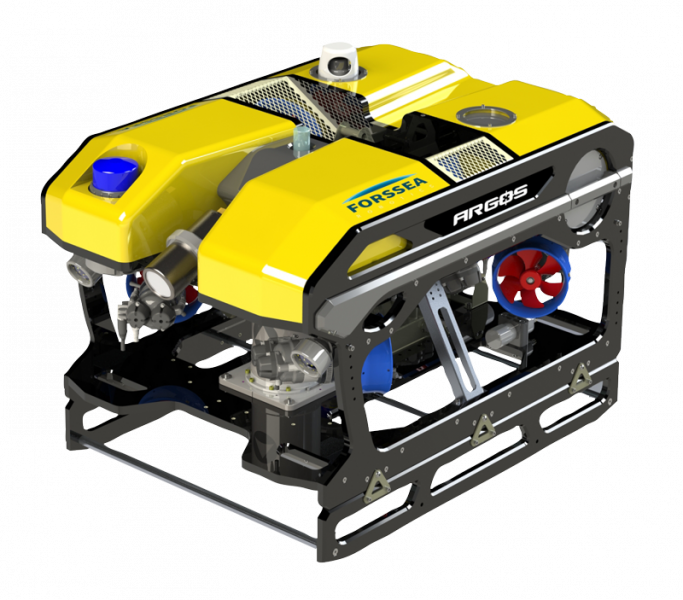
\includegraphics[width=\textwidth]{imgs/Argos.png}
					\caption{\gls{Argos}}
				\end{subfigure}
				\hfill
				\begin{subfigure}[b]{0.3\textwidth}
					\centering
					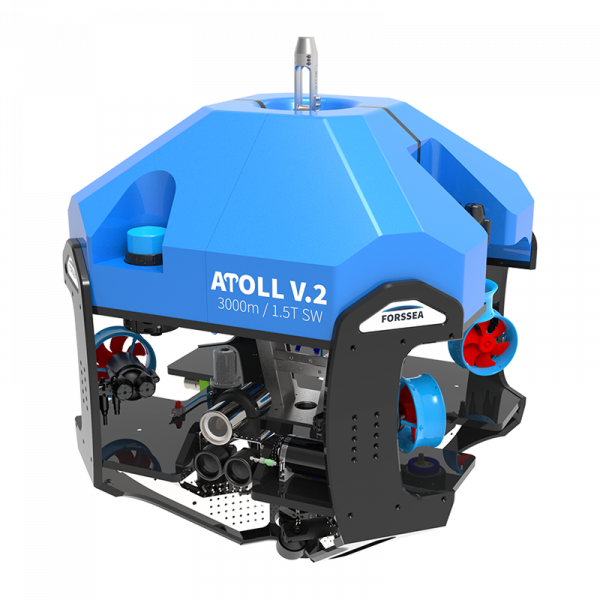
\includegraphics[width=\textwidth]{imgs/Atoll.png}
					\caption{\gls{Atoll}}
				\end{subfigure}
				\hfill
				\begin{subfigure}[b]{0.3\textwidth}
					\centering
					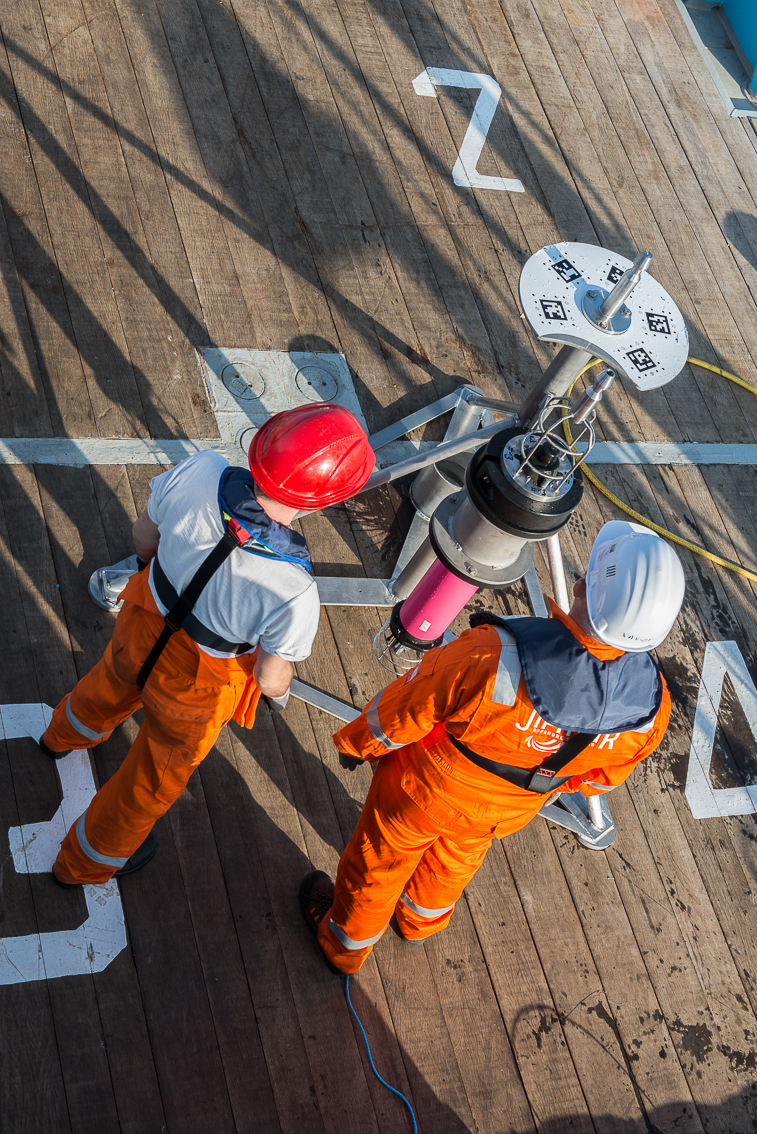
\includegraphics[width=\textwidth]{imgs/Frame.jpg}
					\caption{\gls{frameLBL} et Balise}
				\end{subfigure}
				\caption{\gls{ROV}s proposés par \forssea{} et \gls{frameLBL}}
				\label{fig:ROVs}
			\end{figure}

			Ils proposent aussi plusieurs solutions de captations visuelles\footnote{\url{https://forssea-robotics.fr/index.php/products/cameras}}. Il y a la \gls{Navcam} qui est une caméra embarquant des algorithmes de traitement permettant de réaliser du positionnement visuel, et l'\gls{Obscam} qui est une simple caméra étanche.

	\section[Projet de fin d'études]{Présentation du projet de fin d'études}

		\subsection{Cadre professionnel}

			Ce projet de fin d'étude s'inscrit dans le cadre d'un contrat de professionnalisation réalisé chez Forssea Robotics, entre octobre 2020 et octobre 2021. Il m'a permis d'effectuer un premier pas dans le monde industriel tout en finissant ma formation à l'\gls{ENSTAB}. J'ai donc pu avoir à ma charge un sujet plus complet étant donnée de la durée de ce stage, mais j'ai aussi pu avoir plus de responsabilités dans la gestion de ce projet, dans la mesure ou j'ai intégré l'équipe robotique de \forssea{} pendant une année complète dont six mois à temps plein.

		\subsection{Présentation du sujet}

			Dans les phases de développements des robots, \forssea{} doit faire face à de nombreuses problématiques, dont celle de tester les algorithmes implémentés sur les \gls{ROV}s. Pour cela l'entreprise réalise régulièrement des tests et conditions réelles, mais ce sont des essais coûteux et qui prennent beaucoup de temps à planifier et à organiser. Afin de réduire le nombre d'essais nécessaires, il serait préférable de développer un moyen de test rapide et fiable des robots dans leur environnement. Cela permettrait d'améliorer les performances des robots tout en diminuant les coûts et les temps de développements.

		\subsection{Objectifs du projet}

			L'objectif de ce stage est donc de construire un environnement de simulation sous-marin pour \forssea{}. Il devra permettre de simuler au mieux le comportement des robots dans leur milieu, mais aussi être interfacable avec le reste de l'implémentation logicielle pour tester leurs algorithmes de navigations autonomes. Cet environnement de simulation doit aussi permettre de tester les \gls{ROV}s dans des situations qui peuvent être difficiles à mettre en place lors d'expérimentations. Il est tout de même à noter qu'aucun simulateur ne saurait remplacer la réalisation de tests en conditions réelles.

	